\documentclass[USenglish,a4paper,12pt]{nitathesis}

%%%%%%%%%%%%%%%%%%%%%%%%%%%%%%%%%%%%%%%%%%%%%

\usepackage{tikz}
\usetikzlibrary{shapes.geometric, arrows, positioning, fit, calc, shadows, backgrounds}

\tikzstyle{startstop} = [rectangle, rounded corners, minimum width=3cm, minimum height=1cm,text centered, draw=black, fill=red!30]
\tikzstyle{process} = [rectangle, minimum width=3.5cm, minimum height=1cm, text centered, draw=black, fill=blue!30]
\tikzstyle{decision} = [diamond, minimum width=3.5cm, minimum height=1cm, text centered, draw=black, fill=green!30]
\tikzstyle{arrow} = [thick,->,>=stealth]


\usepackage{xcolor}
\makeatletter
\def\@xfloat #1[#2]{%
  \@nodocument
  \def \@captype {#1}%
   \def \@fps {#2}%
   \@onelevel@sanitize \@fps
   \def \reserved@b {!}%
   \ifx \reserved@b \@fps
     \@fpsadddefault
   \else
     \ifx \@fps \@empty
       \@fpsadddefault
     \fi
   \fi
   \ifhmode
     \@bsphack
     \@floatpenalty -\@Mii
   \else
     \@floatpenalty-\@Miii
   \fi
  \ifinner
     \@parmoderr\@floatpenalty\z@
  \else
    \@next\@currbox\@freelist
      {%
       \@tempcnta \sixt@@n
       \expandafter \@tfor \expandafter \reserved@a
         \expandafter :\expandafter =\@fps
         \do
          {%
           \if \reserved@a h%
             \ifodd \@tempcnta
             \else
               \advance \@tempcnta \@ne
             \fi
           \fi
           \if \reserved@a t%
             \@setfpsbit \tw@
           \fi
           \if \reserved@a b%
             \@setfpsbit 4%
           \fi
           \if \reserved@a p%
             \@setfpsbit 8%
           \fi
           \if \reserved@a !%
             \ifnum \@tempcnta>15
               \advance\@tempcnta -\sixt@@n\relax
             \fi
           \fi
           }%
       \@tempcntb \csname ftype@\@captype \endcsname
       \multiply \@tempcntb \@xxxii
       \advance \@tempcnta \@tempcntb
       \global \count\@currbox \@tempcnta
       }%
    \@fltovf
  \fi
  \global \setbox\@currbox
    \color@vbox
      \normalcolor
      \vbox \bgroup
        \hsize\columnwidth
        \@parboxrestore
        \@floatboxreset
}
\makeatother

\usepackage{graphicx,times,epsfig,amsmath}
\usepackage[square,numbers,comma]{natbib}
\usepackage{amssymb,amsfonts,textcomp}
\usepackage[utf8]{inputenc}
% \usepackage[Sonny]{myfancy}
\usepackage[Sonny]{fncychap}
\usepackage{latexsym}
\usepackage{float}
\usepackage{xspace}
\usepackage{algorithmwh}
\usepackage{comment}
\usepackage{watermark}
\usepackage{graphicx}
\usepackage{pifont}
\usepackage{fancyhdr}
\usepackage{blindtext}
\usepackage{import}
\usepackage{lineno}
\usepackage{rotating}
\usepackage{ragged2e}

% \usepackage{caption}
\usepackage{subcaption}
\usepackage{comment}
\usepackage{nomencl}
\numberwithin{figure}{chapter}
\usepackage{placeins}
\usepackage{relsize}
\usepackage{booktabs}
% \usepackage[nottoc]{tocbibind}
\usepackage{multicol}
\usepackage{multirow}
% \usepackage{rotating}
\usepackage{array}
\usepackage{supertabular}
\usepackage{hhline}
\usepackage{tabularx}
\usepackage{makecell}
\usepackage{verbatim}
\usepackage{chngcntr}
%\usepackage{textcomp}
\usepackage[flushleft]{threeparttable}
\usepackage{tabulary}
% \usepackage{subfig}
% \usepackage{subfigure}
% \usepackage[subfigure]{tocloft}
\usepackage{hyperref}
\usepackage{todonotes}
\hypersetup{
    colorlinks=true,
    linkcolor=blue,
    % filecolor=magenta,      
    % urlcolor=cyan,
}

\emergencystretch=3em
\tolerance=1500


%%%%%%%%%%%%%%%%%%%%%%%%%%%%%%%%%%%%%%%%%%%%%%%%%%%%%
%--reducing the space before the Chapter Headings.

\usepackage{etoolbox}
\makeatletter
\patchcmd{\@makechapterhead}{\vspace*{50\p@}}{\vspace*{0\p@}}{}{}
\patchcmd{\@makeschapterhead}{\vspace*{50\p@}}{\vspace*{0\p@}}{}{}
\makeatother
%%%%%%%%%%%%%%%%%%%%%%%%%%%%%%%%%%%%%%%
%to reduce the spacing 
\usepackage[compact]{titlesec}
\titlespacing{\section}{0pt}{*0}{*0}
 \titlespacing{\subsection}{0pt}{*0}{*0}
\titlespacing{\subsubsection}{0pt}{*0}{*0}

%to reduce the space in itemize/enumerate 
\usepackage{mdwlist}


%Adjusting the space between references in the bibliography.

\newlength{\bibitemsep}\setlength{\bibitemsep}{.2\baselineskip plus .05\baselineskip minus .05\baselineskip}
\newlength{\bibparskip}\setlength{\bibparskip}{0pt}
\let\oldthebibliography\thebibliography
\renewcommand\thebibliography[1]{%
  \oldthebibliography{#1}%
  \setlength{\parskip}{\bibitemsep}%
  \setlength{\itemsep}{\bibparskip}%
}

%%%%%%%%%%%%%%%%%%%%%%%%%%%%%%%%%%%%%%%%%%%%%%%%%%%%%
\counterwithout{footnote}{chapter}
% \usepackage[colorinlistoftodos]{todonotes}
% \usepackage{todonotes}
% \usepackage[draft]{todonotes} 

%\usepackage[square, sort, numbers, authoryear]{natbib}
% \small
\bibliographystyle{abbrv}

% \def\small{\@setsize\small{10pt}\ixpt\@ixpt}
%Table commands
\newcommand\tabletop{\hline\noalign{\smallskip}}
\newcommand\tablemid{\noalign{\smallskip}\hline\noalign{\smallskip}}
\newcommand\tablebot{\noalign{\smallskip}\hline}
\newcommand\tablecline[2]{\noalign{\smallskip}\cline{#1-#2}\noalign{\smallskip}}
\newcommand\kcil[1]{\todo[author=KC,color=red!40,inline]{#1}}
\setlength {\marginparwidth }{2cm} 
%%%%%%%%%%%%%%%%%%%%%%%%%%


%%%%%%%%%%%%%%%%%%%%%%%%%%
\lhead{}
\chead{}
%\rhead{CSED, NIT Agartala}
\lfoot{ }
\cfoot{\thepage}
\rfoot{}

%\setlength{\headrulewidth}{0.4pt}
%\setlength{\footrulewidth}{0.4pt}
\setlength{\headheight}{14.5pt}

\renewcommand{\headrulewidth}{0.5pt}
\renewcommand{\footrulewidth}{0.5pt}



%\usepackage{algorithms}% \Add{} and \Del{} Corrections and \Mark{}
\begin{document}

% Using the watermark package which is in StyleFiles/
% and to remove DRAFT COPY ONLY appearing on the top of all pages comment out below line
%\watermark{SAMPLE COPY ONLY}

\beforepreface
\prefacesection{Acknowledgement}
%%%%%%%%%%%%%%%
%% Here,  write the content of Acknowledgement
%% Blind Text are here for the sample template 
I take this opportunity to express my deep sense of gratitude to all who helped me directly or indirectly during this project work. \\
Firstly, I would like to thank my manager, \textbf{Mr. Vivek Rodge}, for being an exceptional guide and the best advisor I could ever have. His advice, encouragement and constructive feedback are sources of innovative ideas, inspiration and the causes behind the successful completion of this report. His confidence shown to me was the biggest source of inspiration for me. It has been a privilege working with him for the past 6 months.\\ 
I am highly obliged to all the faculty members of the Computer Science and Engineering Department for their support and encouragement. I also thank  \textbf{Prof.(Dr.)~S.~K.~Patra}, Director, NIT Agartala; \textbf{Prof. Mrinal Kanti Debbarma}, H.O.D, CSE Department; and \textbf{Dr. Awnish Kumar}, Assistant Professor, CSE Department, for providing excellent computing and other facilities, without which this work could not achieve its quality goal.\\



%%%%%%%%%%%%%%
\vspace*{0.5cm} 
\hspace*{0.5cm}\textbf{\large - Mainak Dasgupta (22UCS006)}
% \hspace*{1cm}\textbf{\large - Anirban Bhattacharya (21UCS046)}

% \vspace*{0.5cm} 
% \hspace*{0.5cm}\textbf{\large - Rupak Sarkar (21UCS059)}
% \hspace*{2cm}\textbf{\large - Ankan Deb (21UCS187)}
 
%\vspace*{0.5cm} \hspace*{1cm}\textbf{\large - Candidate's Name}

\pagestyle{fancy}
\fancyhead[RO,RE]{\nouppercase\rightmark}
\fancyfoot[C]{\thepage}
\listoffigures
\listoftables
\newpage
\prefacesection{Abstract}
%%%%%%%%%%%%%%%% Enter the content of Abstract here 
Enterprise API connector delivery in telecom environments is often fragmented across contract interpretation, bytecode inspection, manual field mapping, and script-based generation. This thesis presents a technical study of the API Development Tool, a web platform developed during an internship at Amdocs, which unifies this lifecycle in one guided workflow. The system combines a React frontend with a Node.js/Express backend to perform Swagger/OpenAPI parsing, JAR bytecode introspection for EJB metadata extraction, interactive mapping, YAML generation, and automated module creation with Socket.IO-based real-time feedback. Using source-code-level analysis and architectural evaluation, the study examines workflow coverage, parser behavior, persistence and synchronization correctness, security posture, and deployment readiness. Results show strong end-to-end workflow support and identify clear enhancement priorities in authentication, cross-platform generation, and automated testing.


%\afterpreface
%\pagenumbering{roman}                     
%\setcounter{page}{12}
\renewcommand{\headrulewidth}{0.5pt}
\pagestyle{fancy}
\fancyhead[RO,RE]{\nouppercase\rightmark}
\fancyfoot[C]{\thepage}
%\fancyhead[RO,RE]{\thepage}
\tableofcontents
\newpage



% This 13 is for total page before chapters starts
%\pagenumbering{roman}
%\setcounter{page}{11}
\newpage
\pagenumbering{arabic}
\setcounter{page}{1}   

\fancyhf{}
\fancyhead[RO]{\slshape\nouppercase\rightmark{}}
\fancyhead[RE]{\slshape\nouppercase\leftmark{}}
\cfoot{\thepage}
\pagestyle{fancy}
%\fancyhead[ro]{\slshape\nouppercase\thepage}
%\fancyhead[re]{\slshape\nouppercase\thepage}
%\fancyhead[ro,re]{\slshape\nouppercase\thepage}

\flushbottom
\chapter{Introduction}

Enterprise telecom integration teams repeatedly build API connectors that map external REST contracts to internal EJB-based services. The lifecycle is predictable but fragmented: engineers parse OpenAPI/Swagger files, inspect compiled JAR metadata, map request and response fields, prepare YAML configurations, and run generation scripts. In many teams, these steps are handled with separate tools and ad-hoc notes, which increases onboarding time, introduces inconsistency, and raises maintenance cost.

This thesis studies the API Development Tool built during an internship at Amdocs. The platform combines a React 18 frontend~\cite{react_docs} and a Node.js/Express backend~\cite{express_docs} to support specification upload, JAR bytecode introspection, interactive mapping, YAML generation, and connector module generation with Socket.IO~\cite{socketio_docs} progress streaming. Its main contribution is workflow unification: previously disconnected activities become a single, traceable process.

\section{Motivation}

The original connector workflow relied heavily on manual interpretation and undocumented decisions. Engineers used text editors for API contracts, Java tools for class inspection, spreadsheets for mappings, and command-line scripts for generation. This approach consumed time and produced variation in naming, structure, and mapping quality.

Because downstream generation depends on strict YAML structure, mapping errors propagated into generated code and Maven artifacts. The process also lacked a central history of why mappings were chosen, making updates and debugging slow. These issues motivated a guided platform that enforces consistency and records decisions.

Table~\ref{tab:manual_vs_automated} summarises the transition from manual to tool-assisted development.

\begin{table}[H]
\centering
\caption{Comparison of manual and tool-assisted connector development.}
\label{tab:manual_vs_automated}
\small
\begin{tabular}{|p{3.2cm}|p{4.5cm}|p{4.5cm}|}
\hline
\textbf{Aspect} & \textbf{Manual Workflow} & \textbf{Tool-Assisted Workflow} \\
\hline
Specification analysis & Text editors, manual reading & Automated parsing with reference resolution and schema flattening \\
\hline
Service discovery & JAR decompilation in Java IDEs & Browser-based bytecode introspection without JVM \\
\hline
Field mapping & Spreadsheets, ad-hoc notes & Interactive dropdowns with source inference \\
\hline
Configuration authoring & Hand-written YAML files & Automated YAML generation from mapping state \\
\hline
Code generation & Command-line script invocation & One-click generation with real-time streaming \\
\hline
Traceability & Undocumented, scattered files & Full audit trail in database \\
\hline
Consistency & Varies by engineer & Enforced by structured workflow \\
\hline
\end{tabular}
\end{table}

\section{Problem Context}

The platform operates in an existing enterprise environment, not a greenfield system. It must align with a mature digital connector module tree, Maven-based build plugins, compiled client-kit JAR artifacts, and mixed Windows/Linux deployment conditions, including air-gapped production networks.

Accordingly, generated outputs must match fixed directory conventions, such as Swagger files under \texttt{src/\allowbreak main/\allowbreak resources/\allowbreak swagger/} and configs under \texttt{src/\allowbreak main/\allowbreak resources/\allowbreak configs/}. The key challenge is end-to-end continuity: connecting ingestion, introspection, mapping, generation, and synchronisation without breaking enterprise constraints.

\section{Objectives}

This thesis provides a code-level and architecture-level analysis of the platform. It traces how inputs move through frontend, backend, filesystem, and generation layers from specification upload to deployable output.

It also evaluates runtime and deployment behaviour, including Tomcat-hosted frontend delivery, PM2-managed backend operation, certificate handling, and filesystem-centric persistence. The study reports evidence-backed findings across security, reliability, portability, and maintainability, and proposes prioritised improvements.

\section{Method of Study}

The methodology is repository-driven technical analysis. Backend evaluation covers route logic, persistence design, synchronisation routines, and generation orchestration. Frontend evaluation covers workflow components, configuration editing, and API communication.

The Swagger parser, JAR parser, and configuration generator are examined in depth: reference resolution and schema flattening, bytecode and signature parsing, EJB detection, field-path extraction, source inference, and multi-EJB mapping assembly. Conclusions are grounded in observed implementation behaviour.

\section{Report Organisation}

The remaining chapters are organised as follows:

\begin{enumerate}
    \setcounter{enumi}{1}
    \item \textbf{Chapter 2: Purpose and Scope} defines project intent, functional boundaries, and expected outcomes.
    \item \textbf{Chapter 3: Related Works} positions the platform against API-first tooling, code generators, and workflow automation approaches.
    \item \textbf{Chapter 4: System Architecture and Design} details frontend, backend, utilities, synchronisation, generation, and deployment design.
    \item \textbf{Chapter 5: Results and Analysis} presents evidence-based evaluation across workflow coverage, architecture, reliability, security, and portability.
    \item \textbf{Chapter 6: Conclusion and Future Work} summarises contributions and outlines a phased enhancement roadmap.
\end{enumerate}

\flushbottom
\flushbottom
\chapter{Purpose and Scope}

\section{Purpose of the Project}

Enterprise connector delivery in telecom teams was historically fragmented across manual specification reading, JAR inspection, mapping spreadsheets, YAML editing, and script execution. This process produced inconsistent outputs and weak traceability.

The API Development Tool addresses that gap by consolidating the full lifecycle in one guided web application. A React 18 frontend~\cite{react_docs} drives the workflow, and a Node.js/Express backend~\cite{express_docs} manages parsing, persistence, synchronisation, and generation orchestration. The purpose is operationally clear: shorten delivery time, standardise mapping outputs, and preserve an auditable record of all connector decisions.

\section{Functional Scope}

The system scope covers five sequential phases that transform input artifacts into a deployable connector module. Figure~\ref{fig:workflow_lifecycle} shows the artifact flow.

\begin{figure}[H]
\centering
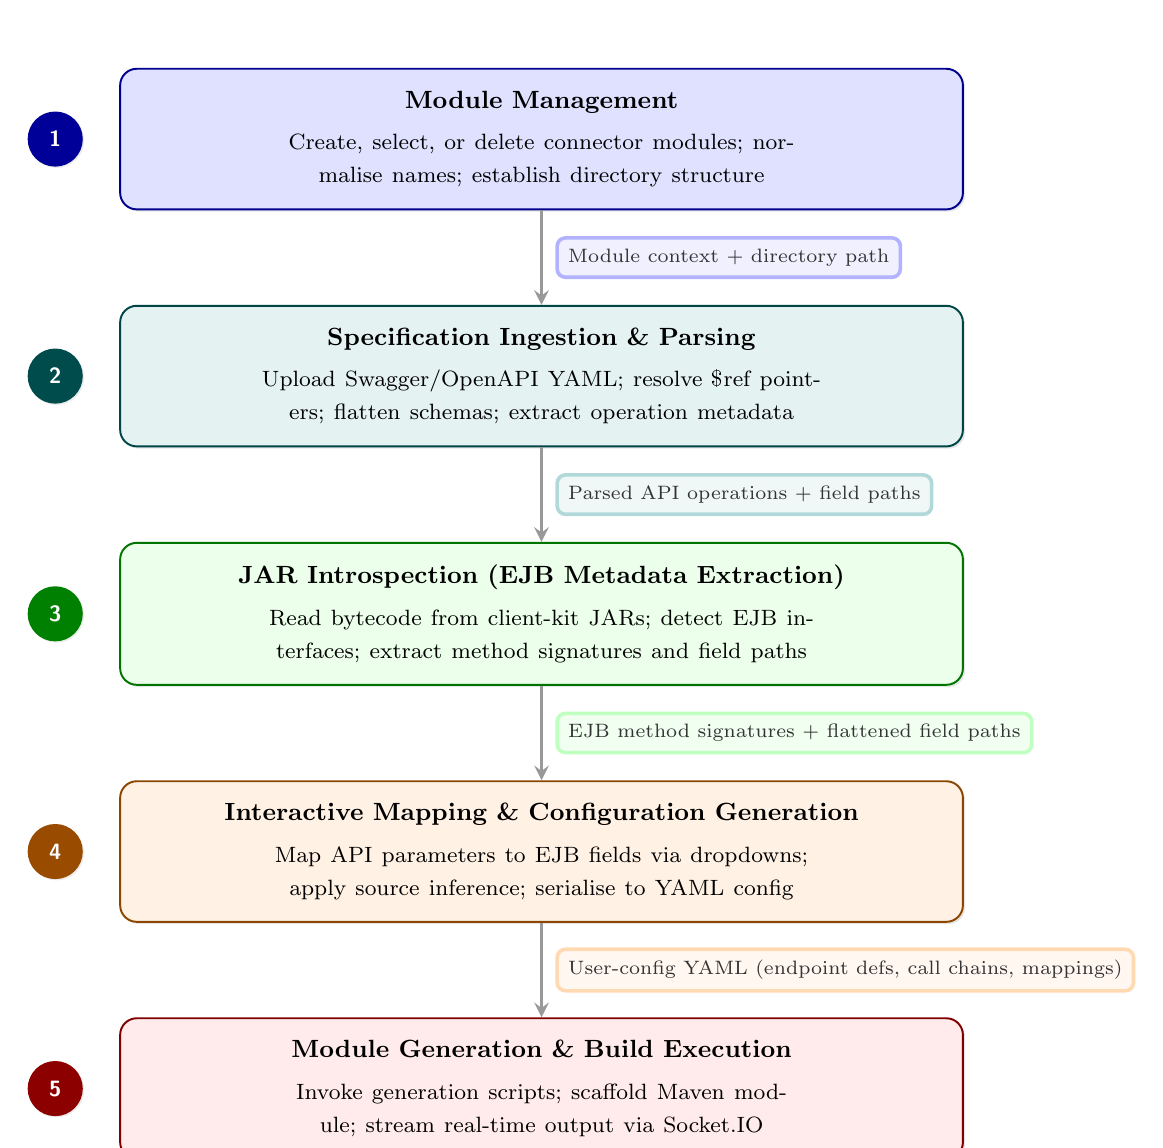
\begin{tikzpicture}[
    phase/.style={rectangle, rounded corners=6pt, line width=0.7pt,
                  text width=10cm, align=center, minimum height=1.5cm,
                  inner xsep=10pt, inner ysep=8pt,
                  drop shadow={shadow xshift=0.8pt, shadow yshift=-0.8pt, opacity=0.2}},
    badge/.style={circle, minimum size=0.7cm, font=\footnotesize\bfseries,
                  text=white, inner sep=0pt, line width=0.7pt,
                  drop shadow={shadow xshift=0.5pt, shadow yshift=-0.5pt, opacity=0.15}},
    arr/.style={->, line width=1.3pt, >=stealth, color=black!40},
    node distance=1.2cm
]

% Phase 1 - Blue
\node[phase, draw=blue!55!black, fill=blue!12] (p1)
    {\textbf{\small Module Management}\\[3pt]
     \footnotesize Create, select, or delete connector modules; normalise names; establish directory structure};
\node[badge, fill=blue!60!black, left=0.45cm of p1.west] {\textsf{1}};

% Phase 2 - Teal
\node[phase, draw=teal!55!black, fill=teal!10, below=of p1] (p2)
    {\textbf{\small Specification Ingestion \& Parsing}\\[3pt]
     \footnotesize Upload Swagger/OpenAPI YAML; resolve \$ref pointers; flatten schemas; extract operation metadata};
\node[badge, fill=teal!60!black, left=0.45cm of p2.west] {\textsf{2}};

% Phase 3 - Green
\node[phase, draw=green!45!black, fill=green!8, below=of p2] (p3)
    {\textbf{\small JAR Introspection (EJB Metadata Extraction)}\\[3pt]
     \footnotesize Read bytecode from client-kit JARs; detect EJB interfaces; extract method signatures and field paths};
\node[badge, fill=green!50!black, left=0.45cm of p3.west] {\textsf{3}};

% Phase 4 - Amber
\node[phase, draw=orange!55!black, fill=orange!10, below=of p3] (p4)
    {\textbf{\small Interactive Mapping \& Configuration Generation}\\[3pt]
     \footnotesize Map API parameters to EJB fields via dropdowns; apply source inference; serialise to YAML config};
\node[badge, fill=orange!60!black, left=0.45cm of p4.west] {\textsf{4}};

% Phase 5 - Red
\node[phase, draw=red!50!black, fill=red!8, below=of p4] (p5)
    {\textbf{\small Module Generation \& Build Execution}\\[3pt]
     \footnotesize Invoke generation scripts; scaffold Maven module; stream real-time output via Socket.IO};
\node[badge, fill=red!55!black, left=0.45cm of p5.west] {\textsf{5}};

% Arrows with colour-matched labels
\draw[arr] (p1.south) -- node[right=5pt, font=\scriptsize, fill=blue!6,
    draw=blue!30, rounded corners=3pt, inner sep=4pt, text=black!80]
    {Module context + directory path} (p2.north);
\draw[arr] (p2.south) -- node[right=5pt, font=\scriptsize, fill=teal!6,
    draw=teal!30, rounded corners=3pt, inner sep=4pt, text=black!80]
    {Parsed API operations + field paths} (p3.north);
\draw[arr] (p3.south) -- node[right=5pt, font=\scriptsize, fill=green!6,
    draw=green!25, rounded corners=3pt, inner sep=4pt, text=black!80]
    {EJB method signatures + flattened field paths} (p4.north);
\draw[arr] (p4.south) -- node[right=5pt, font=\scriptsize, fill=orange!6,
    draw=orange!30, rounded corners=3pt, inner sep=4pt, text=black!80]
    {User-config YAML (endpoint defs, call chains, mappings)} (p5.north);
\end{tikzpicture}
\caption{Five-phase workflow lifecycle of the API Development Tool, showing the key artifacts passed between each phase.}
\label{fig:workflow_lifecycle}
\end{figure}

The phases are:
\begin{enumerate}
    \item \textbf{Module management}: create/select/delete modules and enforce normalised names plus directory conventions.
    \item \textbf{Specification ingestion}: upload Swagger/OpenAPI YAML, resolve references, flatten schemas, and extract operation metadata.
    \item \textbf{JAR introspection}: parse compiled client-kit bytecode, detect EJB interfaces, and extract method and field-path metadata with SHA-256 deduplication.
    \item \textbf{Interactive mapping \& config generation}: map request/response fields (including multi-EJB chains), apply source inference, and generate YAML.
    \item \textbf{Module generation}: invoke the PowerShell-driven generation flow and stream execution output through Socket.IO.
\end{enumerate}

\section{Persistence and Synchronisation}

State is maintained through a hybrid model: sql.js in-process SQLite~\cite{sqljs_docs} for metadata and filesystem storage for artifacts. The core tables are \texttt{swagger\_files}, \texttt{client\_kit\_metadata}, and \texttt{user\_configs}, with unique constraints for duplicate prevention.

Synchronization combines startup reconciliation, runtime chokidar watchers~\cite{chokidar_docs}, and frontend polling fallback. Reconciliation repairs drift between disk and database; watchers detect external file changes; Socket.IO broadcasts keep clients aligned.

\section{Non-Functional Considerations}

The platform supports HTTPS/HTTP modes. In HTTPS mode, it auto-generates self-signed certificates at first startup, which fits air-gapped deployment constraints. The frontend is packaged as a Tomcat WAR~\cite{tomcat_docs}; the backend runs under PM2.

Portability is achieved through relative path resolution and dependency bundling. The stack runs without external database services or runtime internet access. A PowerShell packaging script automates validation, frontend build, WAR creation, and deployable ZIP assembly.

\section{Future Enhancement Opportunities}

The current scope covers the full connector workflow. Planned extensions include authentication and role control, cross-platform generation, stronger automated testing, containerised deployment, and multi-tenant isolation. The existing modular design can support these additions without architectural reset.


\flushbottom
\flushbottom
\chapter{Related Works}

\section{API-First and Contract-Driven Engineering}

API-first engineering treats the API specification as the primary artifact for implementation, testing, and documentation~\cite{openapi_spec}. OpenAPI/Swagger has become the standard contract format for machine-readable endpoint and schema definition.

In contract-driven practice, producer and consumer implementations must remain aligned with that specification. This is critical in enterprise integration, where REST APIs often front legacy EJB-based services. The platform in this thesis follows this model: it parses OpenAPI/Swagger contracts, derives structured metadata, and drives mapping and generation from that contract as the source of truth.

\section{Existing Code Generation Ecosystems}

OpenAPI Generator and Swagger Codegen show that specification-driven scaffolding can accelerate client and server development. They are effective for broad language coverage and template customization.

However, these generators are optimized for generic or greenfield outputs. Enterprise connector environments impose fixed module hierarchies, legacy EJB service contracts, and organization-specific Maven pipelines. Template-based and model-driven approaches remain useful, but they often require substantial adaptation before they fit this context. The examined platform therefore applies a direct contract-to-enterprise transformation flow that combines parsing, metadata extraction, mapping, and generation in one pipeline.

\section{Bytecode Introspection and Metadata Extraction}

The platform's key differentiator is bytecode introspection of compiled client-kit JAR files without source code. Using \texttt{java-class-tools}, it parses class metadata in Node.js/browser environments and avoids JVM-only tooling.

Its extraction depth goes beyond signatures: it resolves hierarchy information, detects EJB interfaces through annotation and naming heuristics, parses generic signatures, flattens nested field paths, and normalizes synthetic parameter names. This output directly supports accurate interactive mapping.

\section{Workflow Automation for Integration Teams}

CI/CD systems automate downstream build and deployment, while low-code integration platforms automate high-level workflow design. Neither category directly addresses the full upstream connector-preparation workflow in legacy EJB environments.

The studied platform sits between these approaches. It offers guided mapping and automation comparable to low-code usability while preserving control required for organization-specific module structures and build chains.

\section{Real-Time Communication in Development Tools}

Real-time feedback is important for long-running generation tasks. Socket.IO~\cite{socketio_docs} provides event messaging, reconnection, and fallback behaviour that fits enterprise network conditions.

In this platform, Socket.IO is used for (i) line-by-line generation log streaming and (ii) state synchronisation events for modules, specifications, client kits, and configurations, with polling fallback for resilience.

\section{Comparison and Positioning}

Existing tools cover fragments of the problem: generic generators focus on code templates, low-code tools focus on abstraction, and CI/CD tools focus on downstream automation. The studied platform combines contract parsing, bytecode extraction, interactive mapping, YAML generation, and scripted module creation in one enterprise-conformant workflow.

Its position is therefore distinct: compiled enterprise artifacts are first-class inputs, outputs match existing module conventions, and users receive real-time operational visibility.

Compared with generic generators, low-code platforms, and CI/CD pipelines, the platform studied here is distinctive in three combined capabilities: bytecode-driven enterprise metadata extraction, interactive contract-to-EJB mapping, and generation output aligned to existing module conventions in air-gapped deployment settings.

\flushbottom
\flushbottom
\chapter{System Architecture and Design}

\section{Overview of the System}

The API Development Tool follows a two-tier client-server model with three functional layers: a React workflow frontend, a Node.js/Express orchestration backend, and an enterprise connector repository containing module structure, scripts, and Maven tooling. Communication is split between REST (CRUD and control operations) and Socket.IO (real-time logs and sync events). The backend links web interactions to filesystem artifacts and external generation scripts. Figure~\ref{fig:system_arch} shows this layered boundary.

\begin{figure}[H]
\centering
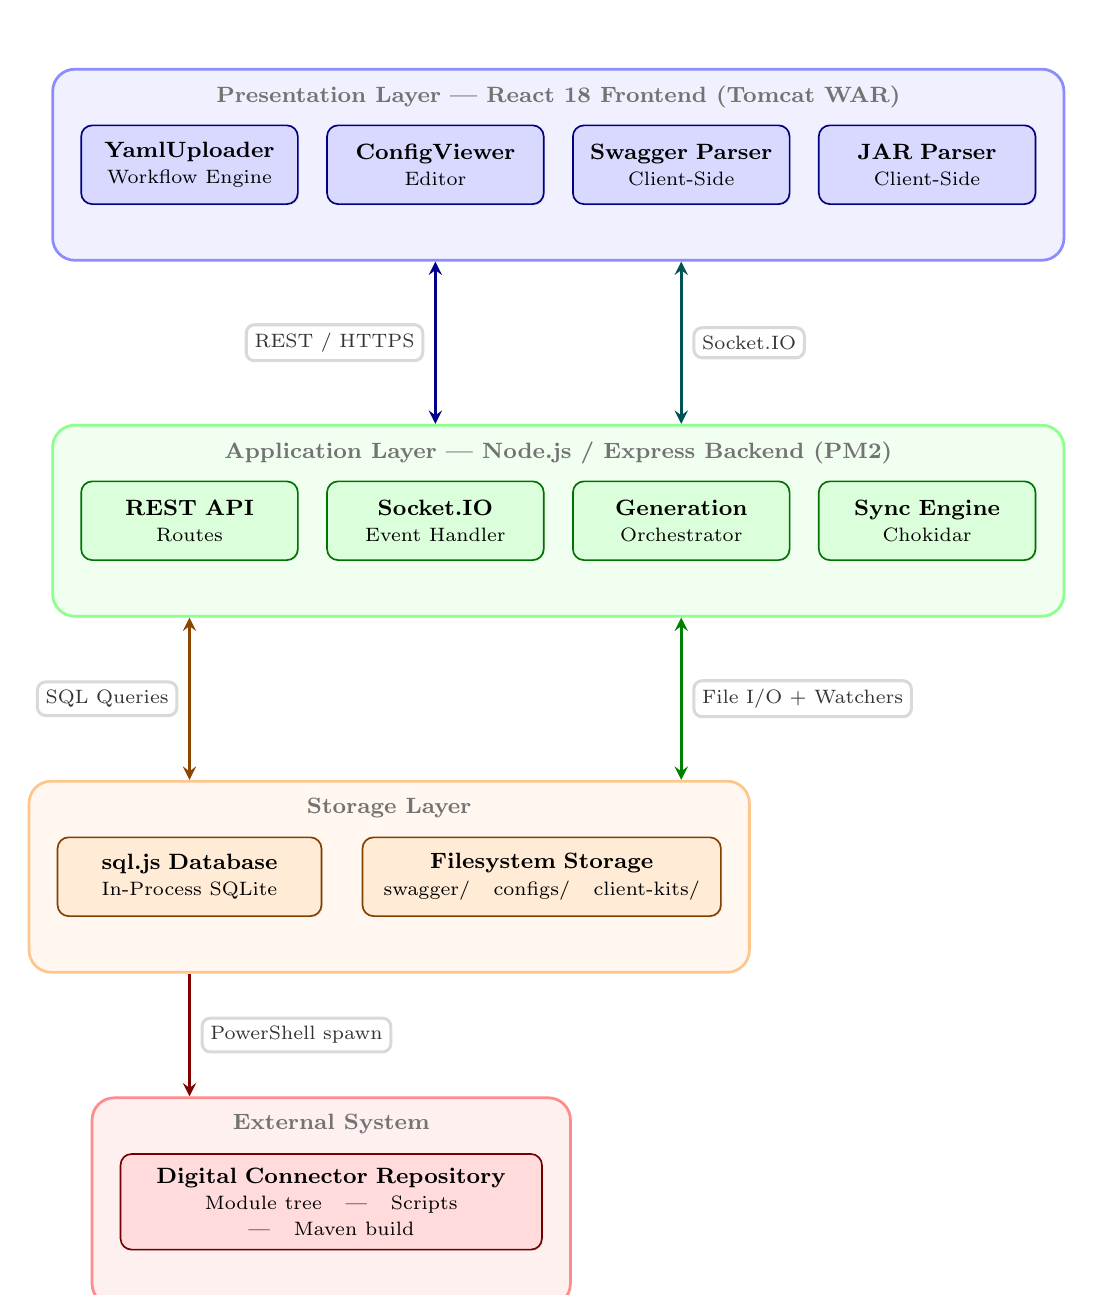
\begin{tikzpicture}[
    comp/.style={rectangle, rounded corners=4pt, line width=0.6pt,
                 text width=2.4cm, align=center, minimum height=1cm,
                 font=\footnotesize, inner sep=5pt,
                 drop shadow={shadow xshift=0.5pt, shadow yshift=-0.5pt, opacity=0.15}},
    layer/.style={rectangle, rounded corners=8pt, draw=#1!45, line width=1pt,
                  inner xsep=10pt, inner ysep=20pt, fill=#1!6},
    layerlbl/.style={font=\footnotesize\bfseries, text=black!55},
    plbl/.style={font=\scriptsize, rounded corners=3pt, inner sep=3pt,
                 text=black!80, fill=white, draw=black!15},
    node distance=0.35cm
]

% --- Presentation Layer components ---
\node[comp, fill=blue!15, draw=blue!50!black] (yu)
    {\textbf{YamlUploader}\\{\scriptsize Workflow Engine}};
\node[comp, fill=blue!15, draw=blue!50!black, right=of yu] (cv)
    {\textbf{ConfigViewer}\\{\scriptsize Editor}};
\node[comp, fill=blue!15, draw=blue!50!black, right=of cv] (sp_c)
    {\textbf{Swagger Parser}\\{\scriptsize Client-Side}};
\node[comp, fill=blue!15, draw=blue!50!black, right=of sp_c] (jp_c)
    {\textbf{JAR Parser}\\{\scriptsize Client-Side}};

% --- Application Layer components ---
\node[comp, fill=green!14, draw=green!45!black, below=3.5cm of yu] (rest)
    {\textbf{REST API}\\{\scriptsize Routes}};
\node[comp, fill=green!14, draw=green!45!black, right=of rest] (sio)
    {\textbf{Socket.IO}\\{\scriptsize Event Handler}};
\node[comp, fill=green!14, draw=green!45!black, right=of sio] (gen)
    {\textbf{Generation}\\{\scriptsize Orchestrator}};
\node[comp, fill=green!14, draw=green!45!black, right=of gen] (sync)
    {\textbf{Sync Engine}\\{\scriptsize Chokidar}};

% --- Storage Layer components ---
\node[comp, fill=orange!16, draw=orange!50!black, below=3.5cm of rest,
      text width=3cm] (db)
    {\textbf{sql.js Database}\\{\scriptsize In-Process SQLite}};
\node[comp, fill=orange!16, draw=orange!50!black, right=0.5cm of db,
      text width=4.2cm] (fstore)
    {\textbf{Filesystem Storage}\\{\scriptsize swagger/ ~ configs/ ~ client-kits/}};

% --- External System ---
\node[comp, fill=red!14, draw=red!45!black, below=3cm of db,
      text width=5cm, xshift=1.8cm] (repo)
    {\textbf{Digital Connector Repository}\\{\scriptsize Module tree ~ | ~ Scripts ~ | ~ Maven build}};

% --- Layer backgrounds (drawn BEHIND components) ---
\begin{pgfonlayer}{background}
\node[layer=blue, fit=(yu)(cv)(sp_c)(jp_c)] (fe_layer) {};
\node[layer=green, fit=(rest)(sio)(gen)(sync)] (be_layer) {};
\node[layer=orange, fit=(db)(fstore)] (st_layer) {};
\node[layer=red, fit=(repo)] (ext_layer) {};
\end{pgfonlayer}

% --- Layer titles INSIDE each box (clear of the inter-layer gaps) ---
\node[layerlbl, anchor=north] at ([yshift=-3pt]fe_layer.north)
    {Presentation Layer --- React 18 Frontend (Tomcat WAR)};
\node[layerlbl, anchor=north] at ([yshift=-3pt]be_layer.north)
    {Application Layer --- Node.js / Express Backend (PM2)};
\node[layerlbl, anchor=north] at ([yshift=-3pt]st_layer.north)
    {Storage Layer};
\node[layerlbl, anchor=north] at ([yshift=-3pt]ext_layer.north)
    {External System};

% --- Protocol-coloured arrows (anchored to component x-positions) ---
\draw[<->, line width=1.1pt, >=stealth, color=blue!55!black]
    (cv.south |- fe_layer.south) --
    node[plbl, left, xshift=-4pt] {REST / HTTPS}
    (cv.south |- be_layer.north);
\draw[<->, line width=1.1pt, >=stealth, color=teal!65!black]
    (sp_c.south |- fe_layer.south) --
    node[plbl, right, xshift=4pt] {Socket.IO}
    (sp_c.south |- be_layer.north);
\draw[<->, line width=1.1pt, >=stealth, color=orange!55!black]
    (rest.south |- be_layer.south) --
    node[plbl, left, xshift=-4pt] {SQL Queries}
    (rest.south |- st_layer.north);
\draw[<->, line width=1.1pt, >=stealth, color=green!50!black]
    (gen.south |- be_layer.south) --
    node[plbl, right, xshift=4pt] {File I/O + Watchers}
    (gen.south |- st_layer.north);
\draw[->, line width=1.1pt, >=stealth, color=red!50!black]
    (db.south |- st_layer.south) --
    node[plbl, right, xshift=4pt] {PowerShell spawn}
    (db.south |- ext_layer.north);

\end{tikzpicture}
\caption{Layered system architecture of the API Development Tool, showing internal subcomponents, communication protocols, and deployment boundaries.}
\label{fig:system_arch}
\end{figure}

\section{Frontend Architecture}

The frontend is a React 18~\cite{react_docs} single-page app with React Router under the \texttt{/retail} base path. The root route hosts \texttt{YamlUploader} (primary workflow), while \texttt{/configs} hosts \texttt{ConfigViewer} (configuration review/editing).

\texttt{YamlUploader} centralizes workflow state for module context, specification data, JAR metadata, mappings, generation status, and console output. It establishes Socket.IO subscriptions and a polling fallback for environments with unstable WebSocket connectivity. Backend calls are wrapped in a unified API service with environment-driven base URL resolution. \texttt{ConfigViewer} reuses parser/generator utilities to keep editing behavior consistent with initial generation.

\section{Utility Layer: Swagger Parser}

The Swagger parser converts OpenAPI/Swagger documents into mapping-ready metadata through three linked steps: \texttt{\$ref} resolution, schema flattening, and operation extraction.

\texttt{\$ref} targets are resolved by traversing JSON pointer segments, with \texttt{WeakMap}-based caching to avoid repeated work. Flattening then produces deduplicated dot-path fields (including arrays and composed schemas via \texttt{allOf}/\texttt{oneOf}/\texttt{anyOf}) with circular-reference protection and depth bounds. Operation extraction combines these results to produce parameter and schema details per endpoint, including precedence-safe merge of path-level and operation-level parameters and support for both Swagger 2.0 and OpenAPI 3.0 request-body styles.

\section{Utility Layer: JAR Parser and Bytecode Introspection}

The JAR parser extracts EJB metadata directly from compiled archives without source code or JVM runtime requirements. Browser and server variants share the same core logic.

JAR files are read via \texttt{jszip}; class files are processed by \texttt{java-class-tools} in batches. The parser decodes JVM descriptors and generic signatures, resolves hierarchy details, and identifies service interfaces using \texttt{javax.ejb.Remote}/\texttt{jakarta.ejb.Remote} annotations plus naming heuristics.

Its critical output is deep, navigable field paths for method inputs and outputs. Recursive traversal includes inherited fields, getter-derived fields, and generic collection element types, bounded by configured depth and path caps for stability. Compiler-generated parameter names are normalized to meaningful names using type-based heuristics.

\section{Utility Layer: Configuration Generator}

The configuration generator converts interactive mappings into YAML required by the generation pipeline. It handles path parameters, request mappings, response mappings, and multi-EJB call ordering.

Request-side logic normalizes target paths (prefix cleanup, array notation, casing), supports source inference for unmapped fields, and rewrites interface-derived prefixes to implementation-compatible paths when needed. Response-side logic filters non-business fields, derives usable nested paths, and supports chained mappings across multiple EJB calls.

The output YAML includes module metadata, generation flags, endpoint definitions, EJB call sequences, and field correspondences, serialized through \texttt{js-yaml}.

The end-to-end transformation is linear and implementation-bound: Swagger/OpenAPI parsing and JAR introspection produce field metadata, interactive mapping resolves source-target correspondences, and the resulting YAML feeds module generation.

\section{Backend Architecture}

The backend is built on Express.js~\cite{express_docs} and combines routing, storage, synchronization, real-time messaging, and generation orchestration in one service. Startup initializes environment variables, storage paths, directories, sql.js schema/migrations, reconciliation routines, and HTTP/HTTPS server plus Socket.IO.

REST endpoints are grouped by domain: modules, Swagger files, client kits, user configs, and generation, with a health endpoint for diagnostics. Metadata persistence uses sql.js~\cite{sqljs_docs} tables (\texttt{swagger\_files}, \texttt{client\_kit\_metadata}, \texttt{user\_configs}) with uniqueness constraints and synchronous export-on-write durability. Validation logic enforces file type and path safety (including path traversal checks) and normalizes module identifiers.

\section{Filesystem Synchronisation}

Consistency between disk state and metadata is maintained in two phases: startup reconciliation and runtime monitoring. Startup routines re-import missing files, remove stale records, and repair drift for modules, client kits, and configs.

At runtime, chokidar~\cite{chokidar_docs} watchers monitor module, client-kit, and config paths with debounced processing and sync coalescing. Confirmed changes trigger database updates and Socket.IO broadcasts (\texttt{modules:sync}, \texttt{swaggers:sync}, \texttt{clientkit:sync}, \texttt{configs:sync}). Generation events (\texttt{generate:start}, \texttt{generate:output}, \texttt{generate:done}) provide live execution visibility.

\section{Module Generation Pipeline}

Generation converts saved Swagger and user-config artifacts into deployable module code. The backend locates the generation script, invokes it through \texttt{spawn}, and supports safe-add (default), force, and optional skip-build modes.

Process output is streamed line-by-line via \texttt{generate:output}, and completion status is emitted through \texttt{generate:done} after success/failure marker checks. A ten-minute timeout protects against hung executions. On platforms without PowerShell, the endpoint returns HTTP 501 while leaving all non-generation features available.

\section{Deployment Architecture}

Deployment uses two services: frontend WAR on Tomcat~\cite{tomcat_docs} and backend Node.js service under PM2. Packaging is automated by a ten-step PowerShell flow covering dependency checks, frontend build, WAR creation, optional smoke tests, and final ZIP bundling.

All runtime paths derive from a configurable digital root, allowing the same codebase to run on Windows and Linux without hardcoded environment-specific paths.

\section{Key Design Decisions}

The implementation prioritizes self-contained deployment, operational transparency, and compatibility with existing enterprise tooling. Filesystem-centric artifact storage plus sql.js export-on-write persistence offers simple auditability and durability for team-scale use.

Workflow state centralization in \texttt{YamlUploader} favors end-to-end usability, while PowerShell-based generation preserves compatibility with established Windows-centric pipelines. Avoiding external database dependencies keeps deployment viable in air-gapped environments.

\flushbottom
\flushbottom
\chapter{Results and Analysis}

\section{Introduction}

This chapter presents the technical evaluation of the API Development Tool based on source-code analysis, architectural review, and runtime behavior. The assessment covers workflow completeness, parser effectiveness, synchronization correctness, security posture, and deployment readiness.

\section{Workflow and Parser Effectiveness}

Backend routes and frontend flow confirm full lifecycle coverage across module management, specification ingestion, JAR introspection, mapping/configuration, and module generation.

Specification parsing supports OpenAPI/Swagger variants, resolves \texttt{\$ref}, flattens composed schemas, and applies correct parameter-precedence rules. JAR parsing handles descriptor and generic-signature decoding, EJB detection by annotation and heuristics, and deep field-path extraction with bounded recursion. Configuration generation produces valid YAML for multi-EJB chains, request/response mappings, and interface-to-implementation path rewriting, with source inference reducing manual effort.

\section{Architecture, Synchronisation, and Persistence}

The two-tier architecture separates frontend workflow concerns from backend orchestration and persistence concerns. Backend endpoints are domain-grouped (modules, Swagger, client-kit, configs, generation), which reduces change impact.

Frontend centralization in \texttt{YamlUploader} provides coherent workflow control and remains decomposable into smaller hooks/components. Utility modules (Swagger parser, JAR parser, configuration generator) are reused across browser/server contexts, reducing behavior drift.

Realtime communication is effective for both generation logging and state synchronization. Socket.IO event streaming, reconnect behavior, startup state emission, debounced watcher handling, and polling fallback provide reliable eventual consistency in enterprise network conditions.

The sql.js layer correctly applies schema setup, migration, and uniqueness constraints. Duplicate prevention for Swagger (file+module) and client-kit content (SHA-256 hash) is enforced at storage level.

Startup reconciliation routines provide self-healing behavior by importing missing files, removing stale records, cascading dependent cleanup, and correcting path drift. Export-on-mutation persistence provides strong durability for the intended team-scale workload.

\section{Security, Deployment, and Portability}

The security model matches its intended trusted-network deployment. Endpoints are open by design, while upload and path handling apply extension checks and traversal-safe path resolution.

Generation requests are validated before script invocation. HTTPS can be enabled via auto-generated self-signed certificates. The architecture can be extended with authentication and stricter CORS if deployment scope expands.

Deployment has been validated in an air-gapped Linux environment, with path-resolution logic supporting both Windows and Linux file conventions. PM2 restart supervision and self-signed HTTPS support improve operational readiness.

Generation depends on PowerShell and therefore degrades gracefully on non-Windows platforms (HTTP 501 for generation while other features remain available). Packaging automation produces a self-contained deployable bundle with pre-check steps.

\section{Consolidated Findings}

The following table summarises the evaluation findings across the key dimensions assessed in this analysis.

\begin{table}[H]
\centering
\caption{Consolidated findings matrix across evaluation dimensions.}
\label{tab:findings}
\begin{tabular}{|p{3.5cm}|p{3.0cm}|p{6.0cm}|}
\hline
\textbf{Dimension} & \textbf{Assessment} & \textbf{Key Observation} \\
\hline
Workflow Coverage & Strong & Complete end-to-end pipeline from specification upload through module generation \\
\hline
Architecture & Good & Clean separation between frontend workflow, backend orchestration, and utility layer \\
\hline
Parsing \& Introspection & Strong & Comprehensive Swagger resolution and deep bytecode field path extraction \\
\hline
Real-time Feedback & Strong & Socket.IO streaming with debounced watchers and polling fallback \\
\hline
Persistence & Good & sql.js with startup reconciliation, hash-based deduplication, and self-healing sync \\
\hline
Security & Appropriate & Trusted-network design with path validation and HTTPS encryption \\
\hline
Portability & Good & Cross-platform path resolution with graceful environment adaptation \\
\hline
Testing & Extensible & Architecture supports progressive addition of test suites \\
\hline
Scalability & Fit for Purpose & Self-contained single-server model optimised for team-scale deployment \\
\hline
\end{tabular}
\end{table}

\section{Performance Observations}

Performance is appropriate for single-user or small-team operation. Swagger parsing is typically sub-second for common specs due to cached reference resolution.

JAR parsing is the dominant computation cost; batching, recursion bounds, and flatten-cache reuse control latency and memory growth. Generation time is mainly external (PowerShell + Maven), commonly tens of seconds to minutes, with real-time streaming reducing perceived wait and timeout guards preventing indefinite hangs.

\flushbottom
\flushbottom
\chapter{Conclusion and Future Work}

\section{Conclusion}

This thesis presented a technical study of an enterprise API connector development platform and confirmed that the implemented workflow is complete, practical, and maintainable for its target environment.

The platform unifies five phases---module management, contract parsing, EJB metadata extraction, mapping/config generation, and module generation---that were previously executed through disconnected tools. The result is improved consistency, lower onboarding effort, and traceable mapping decisions.

Its architecture combines a guided React frontend, an Express orchestration backend, parser/generator utility modules, and real-time feedback via Socket.IO. The hybrid synchronization model (watchers + events + polling fallback) provides resilient behavior under enterprise network constraints. The evaluation also identifies a clear enhancement path for security, portability, storage throughput, and testing depth.

\section{Key Contributions}

The thesis contributes:
\begin{enumerate}
    \item complete architectural documentation of frontend, backend, utility, storage, and generation layers;
    \item algorithm-level analysis of Swagger parsing (\texttt{\$ref} resolution, flattening, operation extraction);
    \item detailed documentation of JAR bytecode introspection (descriptor/signature parsing, EJB detection, deep path extraction, parameter normalization);
    \item evidence-based assessment across reliability, security, portability, and maintainability;
    \item a prioritised roadmap for progressive production hardening.
\end{enumerate}

\section{Future Work}

The platform is functionally mature, but further hardening is required for broader production use. Highest-priority work includes security controls, cross-platform generation support, storage evolution, and automated testing. Medium-priority work includes frontend refactoring and containerized deployment.

\noindent The roadmap is implemented as phased hardening:
\begin{itemize}
    \setlength\itemsep{2pt}
    \item \textbf{Security}: introduce JWT/RBAC, stricter sanitization, and tighter CORS/certificate policies for broader deployment boundaries.
    \item \textbf{Portability}: replace or wrap PowerShell generation with a cross-platform orchestrator while preserving Windows compatibility during transition.
    \item \textbf{Data and quality}: evolve storage for higher concurrency and add unit, integration, and end-to-end automated tests in CI.
    \item \textbf{Maintainability and scale}: decompose \texttt{YamlUploader}, add containerized deployment, and prepare for tenant isolation and queued generation workloads.
\end{itemize}

These enhancements extend the same core architecture and are feasible as incremental releases. The workflow model is also transferable to other regulated integration domains where API-to-enterprise mapping is required and source-code access may be limited.

\section{Summary}

The thesis shows that a workflow-driven connector platform is both technically feasible and operationally valuable in enterprise integration settings. The evaluated implementation delivers strong coverage across parsing, introspection, mapping, generation, synchronization, and deployment.

The roadmap defines incremental next steps that build directly on the current architecture, enabling hardening and scale-up without fundamental redesign.

\flushbottom



\small
\bibliography{bib/mybib}



%%%%%%%%%%%%%%%%%%%%%%%%%%%%%%%%%%%%%%%%%%%%%%%%%%%%%
\appendix


%%%%%%%%%%%%%%%%%%%%%%%%%%%%%%%%%%%%%%%%%%%%%%%%%%%%%
% ographical Sketch\chapter{Publications related to report work}
% \begin{enumerate}	
%  \item  Paper-1 details 
%  \item Paper-2 details
% \end{enumerate}
% % \renewcommand{\thechapter}{\Roman{chapter}}
% % \pagestyle{fancy}
% % \fancyhead[RO,RE]{Bi}
\chapter{Biographical Sketch}
\begin{center}
{\textbf{\large Mainak Dasgupta }}\end{center} %\hrule
\begin{center}
AD Nagar, Agartala, Tripura, PIN-799003,\\ E-Mail: dasguptamainak02@gmail.com,  Contact. No. +91-9366415050 \\
 \end{center}
 \begin{itemize}
  \setlength\itemsep{0pt}
\item Pursuing B.Tech. in Computer Sc. \& Engg. branch from NIT Agartala with CGPA of 7.27.
\item High School from Umakanta Academy (English Medium) under (T.B.S.E), Tripura with 87 \% in 2019.
\item Intermediate from Pranavanada Vidyamandir, under (C.B.S.E), Tripura with 77 \% in 2021.
\end{itemize}
% \newpage
% \begin{center}
% {\textbf{\large Anirban Bhattacharya}}\end{center} %\hrule
% \begin{center}
% Dhaleswar Road no. 16 Agartala, West Tripura PIN-799007,\\E-Mail: bhattacharyaanirban2002@gmail.com,  Contact. No. +91-9863646557 \\
%  \end{center}
%  \begin{itemize}
%  \setlength\itemsep{0pt}
% \item Pursuing B.Tech. in Computer Sc. \& Engg. branch from NIT Agartala with CGPA of 8.59.
% \item Graduated High School from Ramakrishna Mission Vidyalaya,Viveknagar under CBSE with a percentage of 92.6\% in 2021.
% \item Intermediate from Ramakrishna Mission Vidyalaya,Viveknagar under CBSE with a percentage of 95.4 in 2019.
% \end{itemize}

% \begin{center}
% {\textbf{\large Rupak Sarkar}}\end{center} %\hrule
% \begin{center}
% Swami Vivekananda Lane,Bhattapokur,North Badharghat,Agartala,Tripura,PIN-799003 \\E-Mail: kishanrupak1000@gmail.com,  Contact. No. +91-9366059872 \\
%  \end{center}
%  \begin{itemize}
%  \setlength\itemsep{0pt}
% \item Pursuing B.Tech. in Computer Sc. \& Engg. branch from NIT Agartala with CGPA of 9.03.
% \item Completed Class XII Board Examination from Umakanta Academy,Agartala with 92.2\% in 2020.
% \item Completed Class X Board Examination from Chandrai Para Class XII School,Ambassa with 93\% in 2018.
% \end{itemize}

% \begin{center}
% {\textbf{\large Ankan Deb}}\end{center} %\hrule
% \begin{center}
% Taranagar, Sidhai Mohanpur, West Tripura, PIN:799211\\  E-Mail: ankandeb43@gmail.com,  Contact. No. +91-8730842713 \\
%  \end{center}
%  \begin{itemize}
%  \setlength\itemsep{0pt}
% \item Pursuing B.Tech. in Computer Sc. \& Engg. branch from NIT Agartala with CGPA of 9.37.
% \item Completed Higher Secondary from Mohanpur Class XII School,Mohanpur under (T.B.S.E), Tripura with 93.2\% Marks in 2020.
% \item Completed Class X Board Examinations from Mohanpur Class XII School, Mohanpur under (T.B.S.E), Tripura with 94\% Marks in 2018.
% \end{itemize}

\end{document}